\section{A Motivational Study of Verilog Data Contamination}
\label{sec:detection}
\noindent This section conducts an initial audit of widely used Verilog benchmarks and representative Verilog-generation LLMs using existing contamination detectors. The study serves two purposes. First, it examines whether current detectors provide recurring evidence that benchmark samples may have been exposed during model training. Second, and more importantly, it tests whether these detectors are sufficiently consistent to support a credible contamination assessment. As the following results show, multiple detectors repeatedly flag substantial contamination, but their estimated rates disagree so sharply that no individual detector provides a reliable basis for measurement. This observation motivates the controlled evaluation and boosting-based detector introduced in Section~\ref{sec:detector}.
%利用现有方法检测数据污染 并分析实验结果

\subsection{Experimental Setups} \label{sec:target}
We evaluate five representative code-generation LLMs: RTLCoder-Deepseek-v1.1, ChipGPT-Llama2-SFT-7B, Qwen2.5-Coder-7B, DeepSeek-Coder-6.7B-Instruct, and CodeGen-6B-mono. We audit six benchmark variants drawn from VerilogEval, RTLLM, and RealBench~\cite{liu2023verilogeval,lu2024rtllm,jin2025realbench}. VerilogEval and RTLLM each contain two versions, while RealBench is evaluated at the module and system levels. For every model--benchmark pair, we apply the same ten detectors and report both the percentage of samples classified as contaminated and the mean detector score.

\subsection{Existing Detector Configuration} \label{sec:methods}
%各个方法的实验设置

\textbf{Zlib}\ \ The probe concatenates the target model's token probability distribution with the raw input text, compresses the result using the Zlib algorithm, and returns the compression ratio. We set the detection threshold to $-0.003$.

\textbf{Min-K\% Prob}\ \ We used $k=20$ as recommended in the original paper~\cite{shi2024detecting}. The probe computes per-token negative log-likelihood under the target model and returns the average likelihood over the $k\%$ of tokens with the lowest probabilities. Detection threshold was set to $-3.0$.

\textbf{Min-K\%++ Prob}\ \ We used $p=0.2$ as recommended in~\cite{zhang2025min}. The probe extends Min-K\% by incorporating higher-order distributional statistics beyond per-token likelihood. Detection threshold was set to $-3.0$.

\textbf{DC-PDD}\ \ We adopt CodeGen-6B-multi as the reference model and construct a reference corpus of Verilog implementations. This reference corpus is built by collecting Verilog source files from open-source hardware projects. Each entry in the corpus consists of a complete Verilog source file along with its associated metadata (source repository and file path). The corpus contains 5,409 entries, totaling 284 MB. For each input sample, the probe measures distributional discrepancy by comparing the target model's output distribution under two prompt configurations: one conditioned on reference context drawn from this corpus, and one without. We set the detection threshold to $-3.0$.

\textbf{Perplexity}\ \ We computed standard sequence-level perplexity as the exponentiated average negative log-likelihood across all tokens. We set the detection threshold to $-2.2$.

\textbf{PETAL}\ \ We adopt CodeGen-6B-multi as the surrogate model to generate candidate completions, and all-MiniLM-L6-v2 as the sentence embedding model to encode both the generated completions and the original code. The membership score is the cosine similarity between the two embeddings. Samples with scores below $0.8$ are classified as members.

\textbf{Neighbor}\ \ We set $K=5$ neighbors per sample, adopt CodeBERT-base as the MLM backbone for token infilling, and employ two complementary perturbation strategies. For token masking, we set a maximum of 5 masked positions, a span masking probability of 0.7, and top-20 candidates per position. For identifier renaming, we set a renaming probability of 0.6 with a maximum of 3 renames per sample. The maximum sequence length is set to 512 tokens. We set the detection threshold to $0.8$.

\textbf{Reference}\ \ We adopt CodeGen-6B-multi as the reference model, and set the maximum sequence length to 512 tokens and the detection threshold to $0.13$.

\textbf{Token Overlap}\ \ For each sample, the code is split such that the prefix occupies the middle 45--55\% of the token sequence. The target model is prompted with the prefix via in-context learning to generate the completion, and the ROUGE score between the generated completion and the original suffix is returned as the membership score. We enforce minimum prefix and suffix lengths of 120 characters and 4 lines. The maximum generation length is set to 192 tokens, with an ICL context limit of 1,536 tokens. We set the detection threshold to $0.55$.

\textbf{CDD}\ \ For each sample, $N=50$ independent completions are generated under temperature $0.8$ and top-$p$ $1.0$. The statistical test parameters are $\alpha=0.05$ and $\xi=0.01$, with a maximum of 100 tokens compared per generation. Input context is limited to 1,536 tokens and generation to 256 tokens.



\subsection{Preliminary Findings} \label{sec:results}
%基于3个benchmark 5个目标llm 使用10个方法分别进行数据污染检测
%需要的实验结果：
%   1.对于每一对benchmark和llm 检测出的污染样本占比 以及平均检测得分
%   2.做一个热力图相似性分析 具体来说就是 得到一个热力相似性矩阵 行和列分别是10个检测方法 其中矩阵的值 也就是不同方法两两对应的部分 代表这两个方法共同认为该benchmark中污染的样本数量 这样的话最后总共有15个热力图
%   3.根据以上2部分实验 需要得到结论：目前不同数据污染检测方法之间存在明显的不一致现象 无法得出一致的结论 进而提出2个挑战

Table~\ref{tab:detailed_results} presents two complementary findings. On the one hand, several heterogeneous detectors repeatedly classify large fractions of the public benchmarks as contaminated. For example, on RTLCoder-Deepseek-v1.1 with VerilogEval v1, four detectors estimate contamination rates above 90\%. Similarly high estimates recur across different models and benchmark families. Although these uncalibrated outputs cannot establish the true contamination rate, their recurrence provides preliminary evidence that benchmark exposure is not an isolated concern in Verilog generation and warrants systematic investigation.

On the other hand, the estimated rates are dominated by the detector rather than determined consistently by the audited model and benchmark. For RTLCoder-Deepseek-v1.1 on VerilogEval v1, the estimates range from 7.05\% to 100.00\%. For CodeGen-6B-mono on the same benchmark, some detectors report almost no contamination while others classify nearly every sample as contaminated. Even closely related likelihood-based detectors can disagree dramatically: on Qwen2.5-Coder-7B with RTLLM v1, Min-K\% reports 3.45\%, whereas Min-K\%++ reports 100.00\%. The table also exposes systematic detector biases. Perplexity and Min-K\%++ classify nearly all samples as contaminated in many settings, whereas PETAL and Min-K\% frequently produce estimates near zero. Consequently, selecting a different detector can reverse the conclusion of the audit.



\begin{table*}[htbp]
\centering
\caption{Contamination estimates from 10 existing detectors across five models and six benchmark variants. Each entry reports the percentage of samples classified as contaminated.}
\label{tab:detailed_results}
\footnotesize
\renewcommand{\arraystretch}{1.2}
\setlength{\tabcolsep}{2.0pt}   % 收紧列间距，为字体腾空间
\begin{tabular*}{\textwidth}{@{\extracolsep{\fill}} c c *{10}{c} @{}}
\toprule
\rotatebox{30}{\textbf{Model}} & 
\rotatebox{30}{\textbf{Benchmark}} & 
\rotatebox{30}{\textbf{Overlap}} &        % Token Overlap → Overlap
\rotatebox{30}{\textbf{Min-K\%}} & 
\rotatebox{30}{\textbf{Min-K++}} &        % Min-K\%++ → Min-K++
\rotatebox{30}{\textbf{DC-PDD}} & 
\rotatebox{30}{\textbf{PPL}} &            % Perplexity → PPL
\rotatebox{30}{\textbf{Zlib}} & 
\rotatebox{30}{\textbf{Ref.}} &           % Reference → Ref.
\rotatebox{30}{\textbf{Neigh.}} &         % Neighborhood → Neigh.
\rotatebox{30}{\textbf{PETAL}} & 
\rotatebox{30}{\textbf{CDD}} \\
\midrule
% ========== ChipGPT ==========
\multirow{6}{*}{\rotatebox{90}{ChipGPT}} 
& VerilogEval v1   & 17.9  & 19.2  & 100.0  & 35.9  & 100.0  & 19.2 & 66.7  & 46.2  & 12.8  & 12.2  \\
& VerilogEval v2   & 25.6  & 9.0  & 100.0  & 43.6  & 98.1  & 16.7  & 63.5  & 40.4  & 7.1  & 28.8  \\
& RTLLM v1         & 6.9  & 51.7  & 100.0 & 51.7  & 100.0  & 86.2  & 48.3  & 0.0  & 0.0  & 65.5  \\
& RTLLM v2         & 16.0  & 56.0  & 100.0  & 64.0  & 100.0  & 66.0  & 40.0  & 8.0  & 6.0  & 96.0  \\
& RealBench module & 0.0  & 11.7  & 100.0 & 6.7  & 100.0  & 93.3  & 75.0  & 0.0  & 0.0  & 100.0 \\
& RealBench system & 0.0  & 50.0  & 100.0  & 0.0  & 100.0  & 100.0  & 50.0  & 0.0  & 0.0  & 100.0  \\
\midrule
% ========== RTLCoder ==========
\multirow{6}{*}{\rotatebox{90}{RTLCoder}} 
& VerilogEval v1   & 29.5  & 45.5  & 99.4  & 87.2  & 100.0 & 27.6  & 95.5  & 53.8  & 27.6  & 48.7  \\
& VerilogEval v2   & 35.3  & 28.8  & 100.0  & 75.6  & 100.0  & 26.3  & 96.8  & 45.5  & 13.5  &  73.1 \\
& RTLLM v1         & 10.3  & 75.9  & 100.0  & 96.6 & 100.0  & 89.7  & 96.6  & 0.0  & 3.4  & 37.9  \\
& RTLLM v2         & 26.0  & 74.0  & 100.0  & 96.0  &  100.0  & 76.0  & 86.0  & 10.0  & 20.0 & 88.0  \\
& RealBench module & 0.0  & 26.7  & 100.0  & 21.7  & 100.0  & 95.0  & 96.7 & 0.0  & 1.7  & 98.3  \\
& RealBench system & 0.0  & 50.0  & 100.0  & 25.0  & 100.0  & 100.0 & 50.0 & 0.0  & 0.0  & 100.0  \\
\midrule
% ========== OriGen ==========
\multirow{6}{*}{\rotatebox{90}{OriGen}} 
& VerilogEval v1   & 34.6  & 14.7  & 0.0  & 78.2  & 98.1  & 19.9  & 42.9  & 58.3  & 20.5  & 10.9  \\
& VerilogEval v2   & 43.6  & 12.8  & 0.0  & 76.3  & 95.5  & 17.9  & 57.1 & 47.4  & 15.4  & 81.4  \\
& RTLLM v1         & 10.3  & 44.8  & 0.0 & 89.7  & 100.0  & 82.8  & 69.0  & 3.4  & 10.3  & 41.4  \\
& RTLLM v2         & 28.0  & 52.0  & 0.0  & 94.0  & 100.0  & 70.0  & 50.0  & 12.0  & 28.0  & 92.0  \\
& RealBench module & 1.7  & 15.0 & 0.0  & 16.7  & 100.0  & 93.3  & 91.7  & 0.0 & 1.7  & 38.3  \\
& RealBench system & 0.0  & 50.0  & 0.0  & 0.0  & 100.0  & 100.0  & 50.0  & 0.0  & 0.0 & 75.0  \\
\midrule
% ========== VeriCoder ==========
\multirow{6}{*}{\rotatebox{90}{VeriCoder}} 
& VerilogEval v1   & 42.9  & 25.0  & 98.7  & 81.4  & 99.4  & 22.4  & 79.5  & 62.8  & 17.9  & 18.6  \\
& VerilogEval v2   & 40.4  & 10.9 & 99.4  & 67.9  & 96.2 & 18.6  & 69.9  & 48.7  & 10.9  & 49.4  \\
& RTLLM v1         & 13.8  & 48.3 & 100.0  & 89.7  & 100.0  & 79.3  & 65.5  & 6.9  & 6.9 & 0.0  \\
& RTLLM v2         & 24.0  & 54.0  & 100.0  & 94.0  & 100.0  & 70.0 & 60.0  & 18.0  & 20.0  & 88.0  \\
& RealBench module & 1.7 & 15.0  & 100.0  & 18.3  & 100.0  & 90.0  & 93.3  & 3.3  & 3.3  & 53.3  \\
& RealBench system & 0.0  & 50.0  & 100.0  & 25.0  & 100.0  & 100.0  & 50.0  & 0.0  & 0.0  & 100.0  \\
\midrule
% ========== VeriGen ==========
\multirow{6}{*}{\rotatebox{90}{VeriGen}} 
& VerilogEval v1   & 10.3  & 67.3  & 84.0 & 99.4  & 100.0  & 37.2  & 92.9  & 74.4  & 48.1 & 17.9  \\
& VerilogEval v2   & 0.6  & 30.1  & 89.7  & 96.2  & 100.0  & 27.6  & 92.9  & 73.7  & 19.9  & 1.9  \\
& RTLLM v1         & 3.4  & 31.0 & 86.2  & 93.1  & 100.0 & 79.3  & 41.4  & 10.3  & 6.9  & 6.9  \\
& RTLLM v2         & 2.0  & 54.0  & 84.0  & 94.0  & 100.0  & 68.0  & 48.0  & 30.0  & 20.0  & 0.0  \\
& RealBench module & 0.0  & 31.7  & 81.7 & 35.0  & 100.0  & 91.7  & 31.7  & 3.3  & 3.3  & 25.0 \\
& RealBench system & 0.0  & 75.0  & 75.0  & 75.0  & 100.0  & 100.0  & 25.0  & 0.0  & 0.0 & 25.0  \\
\bottomrule
\end{tabular*}
\end{table*}



\begin{figure}[t]
    \centering
    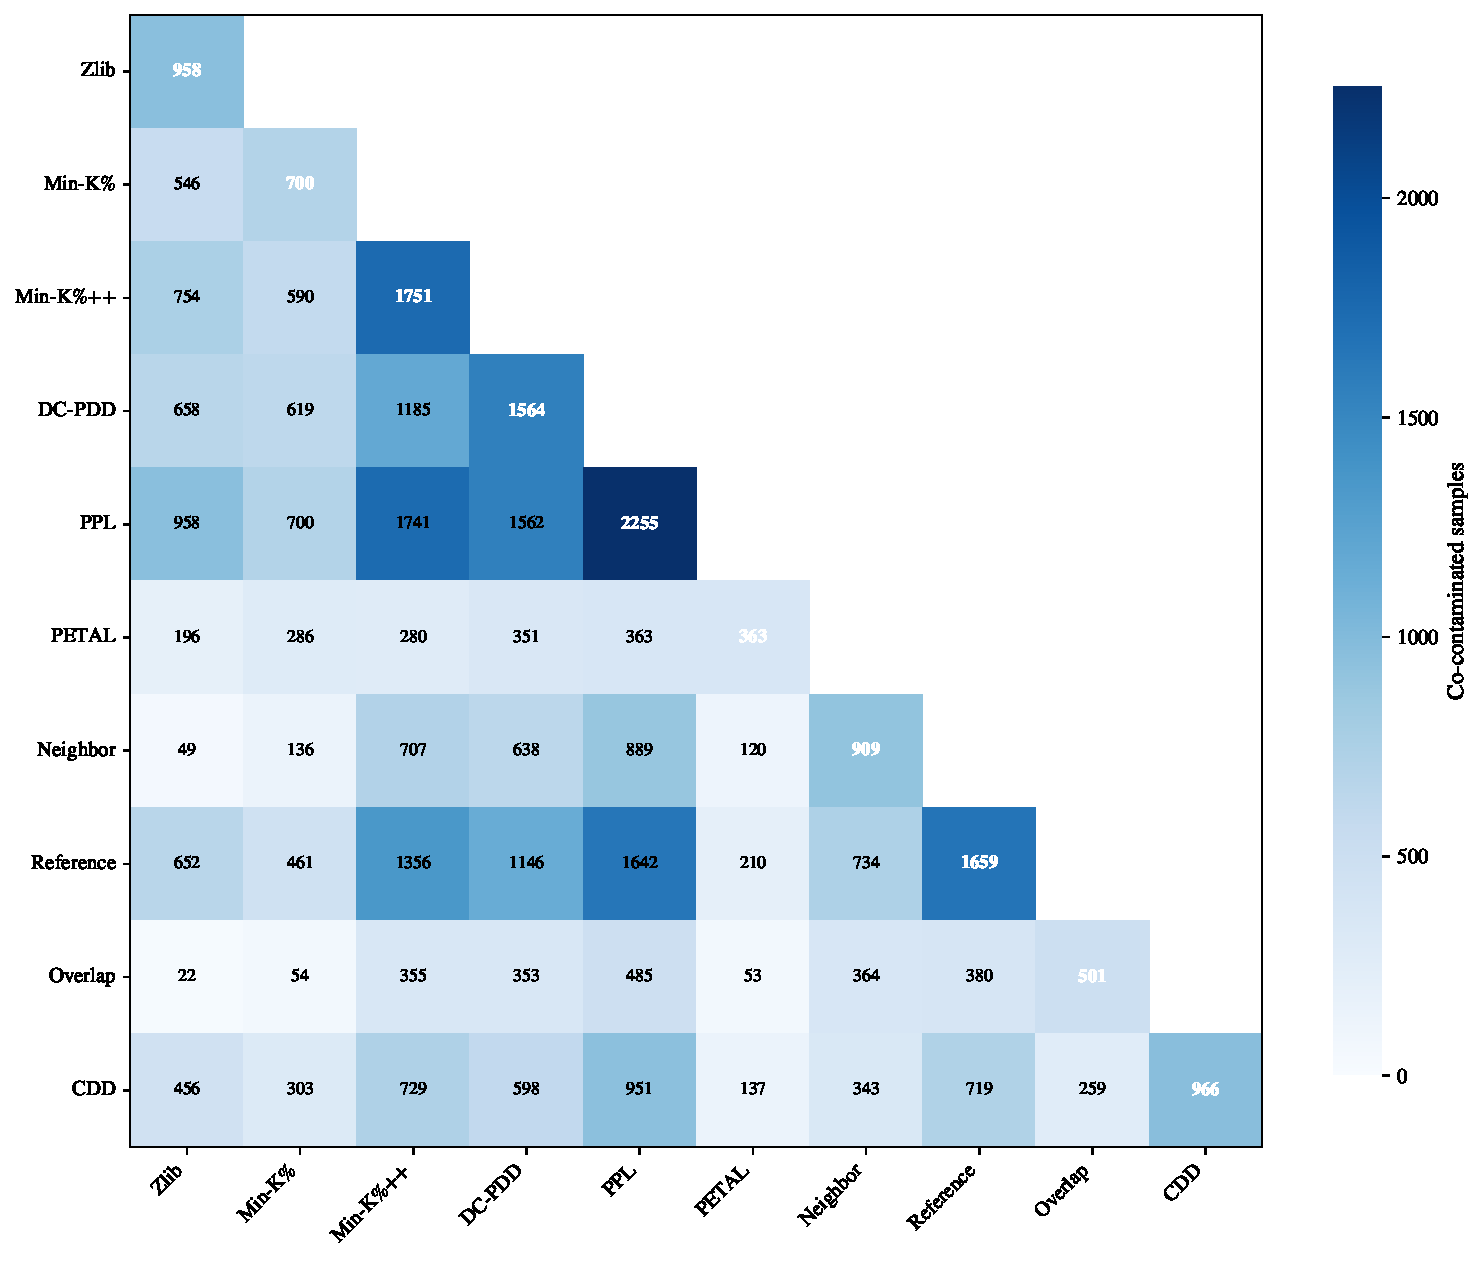
\includegraphics[width=\columnwidth]{figures/overlap_heatmap.pdf}
    \caption{Pairwise overlap between sets of samples flagged as contaminated by different detectors. The variation across detector pairs highlights disagreement at the sample level and suggests potentially complementary detection signals.}
    \label{fig:heatmap}
\end{figure}




\subsection{Implications and Motivation}
\label{sec:motivation}

This study does not treat any single estimate in Table~\ref{tab:detailed_results} as the ground-truth contamination rate. Instead, it establishes two observations that shape the remainder of this work. First, the repeated high estimates produced by multiple detector families indicate that data contamination is sufficiently plausible and widespread to threaten the validity of Verilog benchmark results. Second, the extreme disagreement among detectors prevents those existing methods from quantifying that threat reliably. Reporting the output of a conveniently selected detector would therefore risk either overstating or overlooking contamination.

Beyond the differences in aggregate contamination rates reported in Table~\ref{tab:detailed_results}, Fig.~\ref{fig:heatmap} examines agreement at the sample level through a heatmap of the overlap between the sets of samples flagged as contaminated by different detectors. The overlap varies substantially across detector pairs, showing that the methods disagree on which samples are potentially contaminated as well as on the overall contamination rate. This observation suggests that different detectors may capture different aspects of memorization and consequently identify different subsets of potentially contaminated samples. Their signals may therefore be complementary, motivating an approach that combines evidence from multiple detectors.

The central limitation is the absence of a controlled setting in which the true membership of each sample is known. Without such labels, detector accuracy cannot be measured, thresholds cannot be calibrated for Verilog, and disagreement cannot be resolved. In particular, the sample-level differences in Fig.~\ref{fig:heatmap} do not by themselves establish that the additional samples identified by each detector are truly contaminated. These findings motivate the approach in Section~\ref{sec:detector}: we construct datasets with verified member and non-member samples, evaluate individual detectors against these labels, and learn a boosting-based model that combines their complementary signals into a more reliable contamination estimate.

\begin{comment}
\section{Boosting-Based Data Contamination Detector} \label{sec:detector}

In the previous chapter, we evaluated ten different contamination detection methods across multiple Verilog benchmarks and large language models. Their substantial disagreement shows that relying on any individual probe can lead to unreliable contamination estimates, motivating a detector that combines complementary evidence under a controlled validation framework.

\subsection{Motivation and Problem Formulation}

Given the considerable disagreement among existing detection methods, a natural question arises: can we combine multiple complementary probes to obtain a more reliable and robust contamination indicator? The core difficulty is that for most deployed LLMs, we do not have ground-truth knowledge of which test samples were truly part of the training set. For certain models whose fine-tuning datasets are open-sourced, we can construct a golden dataset, i.e., a collection of samples with known membership status. Such a golden dataset enables us to evaluate and calibrate the behavior of different probes on a per-model basis.

More formally, let $\mathcal{M}$ be a target LLM with a publicly available training set. We construct a golden dataset $\mathcal{D}_{\text{golden}} = \{ (\mathbf{x}_i, y_i) \}_{i=1}^{N}$, where $\mathbf{x}_i$ is an Instruction-Response pair (corresponding to the command and the code, respectively) and $y_i \in \{0,1\}$ indicates whether $\mathbf{x}_i$ belongs to the training set of $\mathcal{M}$ ($y_i=1$) or not ($y_i=0$). For each sample $\mathbf{x}_i$, we compute a feature vector $\mathbf{f}_i = [f_{i,1}, f_{i,2}, \dots, f_{i,K}]$ consisting of the raw scores produced by $K$ different contamination detection probes (e.g., Token Overlap, Min-K\%, Zlib, etc.). These raw scores are then normalized to zero mean and unit variance to remove scale differences across probes.

We treat the contamination detection problem as a supervised binary classification task: given the feature vector $\mathbf{f}_i$, predict the membership label $y_i$. The key challenge is that the relationship between probe scores and true membership is often complex and non-linear. A single probe may perform well on some types of samples but poorly on others, and different probes may capture complementary signals. Therefore, we propose to learn a fusion model that combines the strengths of multiple probes.

Specifically, we adopt a boosting-based ensemble approach. Boosting sequentially trains weak learners (e.g., decision stumps) on re-weighted versions of the training data, where each new learner focuses on the samples that previous learners misclassified. This framework is well-suited for our problem because it can automatically learn non-linear interactions among probes and produce a single, interpretable contamination score. 


\subsection{Golden Dataset Construction}
We construct a labeled dataset from two Verilog-generating models: RTLCoder-Deepseek-v1.1 and CodeV. RTLCoder-Deepseek-v1.1is a state-of-the-art Verilog code generation model fine-tuned from DeepSeek-Coder-v1.5 on a corpus of approximately 55,000 instruction--code pairs generated via GPT-based data synthesis. CodeV is a Verilog-specific model trained on a curated collection of open-source Verilog designs from GitHub and textbooks. These two models represent distinct fine-tuning regimes and architectural lineages, making them suitable candidates for cross-model contamination analysis.

For each model, we collect $500$ contaminated positive samples that are confirmed to be part of the model's fine-tuning data, and $500$ clean negative samples that are independently verified to be absent from its training corpus. A sample is labeled as contaminated if the exact Verilog module code appears in the model's verified training set; it is labeled as clean if the code originates from a held-out source with no overlap with the training data. All samples are structured as instruction--response pairs, where the instruction is a natural language Verilog design specification and the response is the corresponding module implementation. This pairing reflects the standard format in which instruction-tuned code generation models consume training data.

For each sample, all ten probe scores are computed using the corresponding model as the computation backend. That is, features associated with RTLCoder are derived with RTLCoder-Deepseek-v1.1 serving as the model under which loss, perplexity, and generation-based signals are evaluated, while features associated with CodeV employ CodeV as the backend. This per-model computation ensures that each feature vector faithfully captures the internal representation of the model being audited, rather than imposing an external reference model's perspective.

For the cross-model detection experiments described in Section~\ref{sec:detector}, RTLCoder-Deepseek-v1.1 serves as the source model and CodeV as the target model. For the source model, $400$ contaminated and $400$ clean samples are allocated to the training set, while the remaining $100$ per class are reserved for in-domain validation. The entire $1{,}000$ samples of the target model CodeV constitute the out-of-domain test set and are never exposed during training, normalization, or threshold selection.



\subsection{Model Architecture and Training Strategy}

\paragraph{Two-Level Stacking Architecture.}
We adopt a two-level stacking ensemble~\cite{wolpert1992stacked} that integrates the ten probe scores into a unified contamination prediction. The first level employs three gradient-boosted tree models selected for their complementary inductive biases:

\begin{itemize}
\item \textbf{XGBoost}~\cite{chen2016xgboost}: 700 estimators with a maximum depth of 4 and a learning rate of 0.03. Both subsample and column sampling ratios are set to 0.9. The level-wise tree growth with $\ell_2$ regularization ($\lambda = 1.0$) provides stable gradient estimates.
\item \textbf{LightGBM}~\cite{ke2017lightgbm}: 900 estimators with 31 leaves per tree and a learning rate of 0.02. The leaf-wise growth strategy with gradient-based one-side sampling captures fine-grained feature interactions that XGBoost may miss.
\item \textbf{CatBoost}~\cite{prokhorenkova2018catboost}: 900 iterations with a maximum depth of 6 and a learning rate of 0.03. Its ordered target encoding reduces prediction shift caused by target leakage in the boosting process, offering a complementary perspective to the other two base learners.
\end{itemize}

Each base learner produces an out-of-fold (OOF) prediction probability via a 5-fold stratified cross-validation procedure, ensuring that no training sample contributes to both model fitting and meta-feature construction. The three OOF predictions serve as meta-features for the second-level classifier:

\begin{equation}
    \hat{y} = \sigma\!\left(\mathbf{w}^{\top} \cdot \frac{\mathbf{x}_{\text{meta}} - \boldsymbol{\mu}}{\boldsymbol{\sigma}} + b\right),
    \label{eq:meta}
\end{equation}

where $\mathbf{x}_{\text{meta}} = [\,p_{\text{XGB}},\, p_{\text{LGB}},\, p_{\text{CAT}}\,]$ is the vector of base-learner outputs, $\boldsymbol{\mu}$ and $\boldsymbol{\sigma}$ are the element-wise mean and standard deviation estimated from the training meta-features, and $\sigma(\cdot)$ denotes the logistic sigmoid. Standardization of the meta-features before logistic regression stabilizes convergence and places the three base models on a comparable scale. The final decision threshold $\tau$ is set by maximizing classification accuracy on the OOF predictions:

\begin{equation}
    \tau^* = \mathop{\arg\max}_{\tau \in [0.05,\,0.95]} \; \text{Accuracy}\!\left(\mathbf{y}_{\text{train}},\; \mathbf{1}\!\left[\hat{\mathbf{y}}_{\text{OOF}} \geq \tau\right]\right).
    \label{eq:threshold}
\end{equation}

The choice of sweeping $\tau$ over $[0.05, 0.95]$ with a granularity of $0.005$ balances precision against computational cost; coarser grids yield nearly identical thresholds in practice.

\paragraph{Cross-Model Generalization Formulation.}
We formulate data contamination detection as a cross-model generalization problem. The detector is trained exclusively on labeled data from a source model and subsequently applied to a distinct target model whose training corpus is assumed inaccessible. This formulation mirrors the practical scenario in which one wishes to audit whether a third-party model, for which only the model weights or inference API are available, has been trained on specific benchmark datasets.

\paragraph{Per-Model Z-Score Normalization.}
A critical obstacle in cross-model contamination detection is the distributional shift of probe scores across different model backends. The same code snippet, when evaluated under two different language models, can yield probe scores on substantially different numerical ranges. For instance, a zlib compression ratio of $-0.003$ may indicate strong memorization under RTLCoder, while the same threshold applied to CodeV could classify nearly all samples as uncontaminated due to systematic differences in the models' compression characteristics. Consequently, a detector trained on raw source-model features is unlikely to transfer to a target model without explicit distribution alignment.

To mitigate this issue, we apply per-model z-score normalization independently to the features of each model. Let $\mathbf{x}_i^{(m)} \in \mathbb{R}^{10}$ denote the probe score vector for the $i$-th sample computed using model $m$ as the backend. The normalization is performed as:


\begin{equation}
    \tilde{\mathbf{x}}_i^{(m)} = \frac{\mathbf{x}_i^{(m)} - \bar{\mathbf{x}}^{(m)}}{\boldsymbol{\sigma}^{(m)}},
    \label{eq:zscore}
\end{equation}


where $\bar{\mathbf{x}}^{(m)} = \frac{1}{N_m} \sum_{i=1}^{N_m} \mathbf{x}_i^{(m)}$ and $(\boldsymbol{\sigma}^{(m)})_j = \big(\frac{1}{N_m} \sum_{i=1}^{N_m} (x_{i,j}^{(m)} - \bar{x}_j^{(m)})^2 \big)^{1/2}$ for each feature dimension $j$. Division-by-zero is handled by replacing zero-valued standard deviations with unity, which occurs only for constant-valued features that carry no discriminative information.


This transformation expresses each score in units of standard deviation relative to the corresponding model's typical output distribution. After normalization, a zlib score of $+2.0$ on both RTLCoder and CodeV carries the same semantic interpretation: the sample is two standard deviations above the respective model's average compression ratio. Empirically, we find that omitting this normalization step degrades the out-of-domain AUC by up to $0.12$ on certain model pairs, underscoring its importance for cross-model transfer.

\paragraph{Training Procedure.}
The complete training procedure is formalized in Algorithm~\ref{alg:training}. We emphasize that neither the target model's feature distributions, labels, nor any sample-level statistics from CodeV are accessible during training. This constraint rigorously evaluates whether the contamination detection patterns learned from one model generalize to a different model architecture.



\begin{algorithm}[t]
    \caption{Cross-Model Detector Training}
    \label{alg:training}
    \begin{algorithmic}[1]
        \Require Source model $M_s$, labeled data $\mathcal{D}_s = \lbrace(\mathbf{x}_i^s, y_i)\rbrace_{i=1}^{N_s}$; target model $M_t$, unlabeled data $\mathcal{D}_t = \lbrace\mathbf{x}_j^t\rbrace_{j=1}^{N_t}$
        \Ensure Trained stacking detector $\mathcal{F}$ and threshold $\tau^*$
        \State Compute normalization parameters $\bar{\mathbf{x}}^s, \boldsymbol{\sigma}^s$ from $\mathcal{D}_s$ via Eq.~\eqref{eq:zscore}
        \State Normalize: $\mathbf{x}_i^s \leftarrow (\mathbf{x}_i^s - \bar{\mathbf{x}}^s) \;/\; \boldsymbol{\sigma}^s$ for all $i$
        \State Initialize base models: $\mathcal{M}_1$ (XGBoost), $\mathcal{M}_2$ (LightGBM), $\mathcal{M}_3$ (CatBoost)
        \State Generate 5-fold stratified CV splits $\lbrace\text{fold}_k\rbrace_{k=1}^5$ on $\mathcal{D}_s$
        \For{$k = 1$ to $5$}
            \State $\mathcal{D}_{\text{train}}^{(k)} \leftarrow \mathcal{D}_s \setminus \text{fold}_k$, \quad $\mathcal{D}_{\text{val}}^{(k)} \leftarrow \text{fold}_k$
            \For{$m = 1$ to $3$}
                \State Train $\mathcal{M}_m$ on $\mathcal{D}_{\text{train}}^{(k)}$
                \State Collect OOF predictions: $\hat{\mathbf{y}}_{\text{OOF}}^{(m)}[\text{fold}_k] \leftarrow \mathcal{M}_m\text{.predict\_proba}(\mathcal{D}_{\text{val}}^{(k)})$
            \EndFor
        \EndFor
        \State Build meta-features: $\mathbf{X}_{\text{meta}} \leftarrow \big[\,\hat{\mathbf{y}}_{\text{OOF}}^{(1)},\; \hat{\mathbf{y}}_{\text{OOF}}^{(2)},\; \hat{\mathbf{y}}_{\text{OOF}}^{(3)}\,\big]$
        \State Train meta-classifier $\mathcal{F}_{\text{meta}}$ (Logistic Regression) on $(\mathbf{X}_{\text{meta}}, \mathbf{y})$
        \State Select $\tau^*$ by maximizing accuracy on $\mathcal{F}_{\text{meta}}\text{.predict\_proba}(\mathbf{X}_{\text{meta}})$ via Eq.~\eqref{eq:threshold}
        \State \Return $\mathcal{F} = \lbrace\mathcal{M}_1, \mathcal{M}_2, \mathcal{M}_3, \mathcal{F}_{\text{meta}}\rbrace$ and $\tau^*$
    \end{algorithmic}
\end{algorithm}
\end{comment}

\section{Boosting-Based Data Contamination Detector}
\label{sec:detector}

The motivational study in Section~\ref{sec:detection} shows that no individual detector provides a consistently reliable contamination estimate for Verilog. We therefore turn to a controlled setting with known membership labels and learn to combine the complementary evidence captured by different detectors.

\subsection{Problem Formulation}
\label{sec:formulation}

We formulate data contamination detection as a binary classification problem. For LLM $\mathcal{M}$, define a golden dataset $\mathcal{D} = \{ (\mathbf{c}_i, y_i) \}_{i=1}^{N}$(Section~\ref{sec:golden_dataset}), where $\mathbf{c}_i$ denotes an Prompt--Response pair, and $y_i \in \{0, 1\}$ indicates whether $\mathbf{c}_i$ belongs to the training set of $\mathcal{M}$.Our objective is to learn a function $f(x) \in [0,1]$ that outputs the contamination probability for $\mathbf{c}_i$, and subsequently predict whether it is contaminated by applying a threshold learned during training. The function $f$ will be implemented as a boosting ensemble that combines the outputs of multiple base methods introduced in Section~\ref{sec:detection}.



\subsection{Golden Dataset Construction}
\label{sec:golden_dataset}

We construct three golden datasets corresponding to three LLMs including \textbf{CodeV-DS-6.7B}~\cite{zhao2024codev}, \textbf{RTLCoder-Deepseek-v1.1}~\cite{liu2024rtlcoder}, and \textbf{OriGen}~\cite{cui2024origen}. All of them are Verilog-generation models fine-tuned on domain-specific instruction data. Each golden dataset is a balanced binary-labeled collection of Verilog code snippets, where a positive label indicates that the snippet is known to be present in the model's training set, and a negative label indicates the opposite.

\textbf{Positive Samples.} For each model, we select 500 Verilog code entries from its respective fine-tuning training corpus. Since these entries are explicitly included in the model's training data, they constitute a clean contaminated set such that any detection method correctly identifying them as contaminated yields a true positive by construction. This design provides a reliable ground-truth for the positive class.

\textbf{Negative Samples.} Negative samples are drawn from the \textbf{hdl2v} open-source training corpus~\cite{hong2025hdl2v}, a dataset released in 2025 that comprises Verilog code automatically translated from VHDL designs. From this corpus, we select the translated Verilog code, and synthetically generate natural language descriptions  for each Verilog entry using \textbf{DeepSeek-V4}~\cite{xu2026deepseek}. We apply a filtering procedure during selection to exclude entries with excessive length, incomplete syntax, or anomalous formatting. Unlike conventional Verilog datasets collected from public GitHub repositories, hdl2v is synthetically generated through translation, meaning its core Verilog contents do not exist in any open-source repository and thus could not have been inadvertently scraped. To provide an additional layer of guarantee, we performed a systematic deduplication check against the training corpora of all three target models, confirming that none of the selected entries appear in any of their fine-tuning sets. From this corpus, we select a total of 1,500 Verilog entries after filtering, and randomly assign 500 entries to each of the three models as negative samples.

\textbf{Dataset Split.} The 1,000-sample dataset for each model is split into an 800-sample training set and a 200-sample test set, both maintaining the 1:1 positive-to-negative ratio. Across all three models, this yields a total of 2,400 training samples and 600 test samples. The three test sets are used independently in Section~\ref{sec:evaluation} to evaluate both the individual methods and the proposed boosting ensemble.

% Queue Table II before Section IV-C so that it appears at the top of page 6.
\begin{table*}[t]
\centering
\caption{Contamination detection on DeepSeek-Coder-v1.5 variants: AUC-ROC and F1 comparison of individual detectors and the CatBoost ensemble on CodeV, RTLCoder, and OriGen.}
\label{tab:compare_baseline}
\small
\begin{tabularx}{\textwidth}{l *{8}{>{\centering\arraybackslash}X}}
\toprule
& \multicolumn{2}{c}{\textbf{CodeV}} & \multicolumn{2}{c}{\textbf{RTLCoder}} & \multicolumn{2}{c}{\textbf{OriGen}} & \multicolumn{2}{c}{\textbf{Average}} \\
\cmidrule(lr){2-3} \cmidrule(lr){4-5} \cmidrule(lr){6-7} \cmidrule(lr){8-9}
\textbf{Method} & AUC & F1 & AUC & F1 & AUC & F1 & AUC & F1 \\
\midrule
Zlib  & 0.609 & 0.699 & 0.602 & 0.713 & 0.684 & 0.689 & 0.631 & 0.700 \\
Min-K\%  & 0.756 & \uline{0.743} & 0.805 & \uline{0.776} & 0.813 & \uline{0.761} & 0.791 & \uline{0.760} \\
Min-K\%++  & 0.649 & 0.682 & 0.794 & 0.755 & 0.547 & 0.674 & 0.663 & 0.703 \\
DC-PDD  & \uline{0.818} & 0.658 & \uline{0.854} & 0.658 & \uline{0.878} & 0.678 & \uline{0.850} & 0.665 \\
Perplexity  & 0.743 & \uline{0.743} & 0.794 & 0.757 & 0.819 & \uline{0.761} & 0.785 & 0.754 \\
PETAL  & 0.681 & 0.664 & 0.808 & 0.658 & 0.794 & 0.658 & 0.761 & 0.660 \\
Neighborhood  & 0.560 & 0.676 & 0.653 & 0.731 & 0.606 & 0.706 & 0.606 & 0.704 \\
Reference  & 0.753 & 0.734 & 0.557 & 0.687 & 0.648 & 0.691 & 0.653 & 0.704 \\
Token-Overlap  & 0.503 & 0.600 & 0.597 & 0.669 & 0.663 & 0.702 & 0.588 & 0.657 \\
CDD & 0.707 & 0.177 & 0.582 & 0.451 & 0.783 & 0.718 & 0.690 & 0.448 \\
Boost Ensemble & \textbf{0.917} & \textbf{0.859} & \textbf{0.912} & \textbf{0.859} & \textbf{0.951} & \textbf{0.899} & \textbf{0.927} & \textbf{0.872} \\
\bottomrule
\end{tabularx}
\end{table*}

\subsection{CatBoost Ensemble Training}
\label{sec:catboost}

Following the problem formulation in Section~\ref{sec:formulation}, we now describe the training of our ensemble detector. For each code entry, we apply a subset of five methods in Section~\ref{sec:methods}~— DC-PDD, Reference, Neighborhood, Min-K\%, and Zlib~— to obtain a 5-dimensional raw score vector \(\mathbf{s} = [s_1, s_2, \ldots, s_5]\). The scores from different methods operate on distinct numerical ranges; rather than applying normalization, we feed the raw concatenated scores directly into the ensemble model. This preserves the absolute magnitude information of each method, which carries discriminative signal about contamination strength.

We adopt \textbf{CatBoost}~\cite{prokhorenkova2018catboost} as our boosting algorithm. We choose CatBoost over alternative implementations for three reasons: (1) its ordered target encoding eliminates prediction shift, which is critical when transferring a detector trained on source models to unseen target models; (2) its symmetric tree structure provides implicit regularization that prevents overfitting to source-model-specific patterns; and (3) its scale-invariant tree splits eliminate the need for per-model feature normalization, as decision boundaries learned via absolute thresholds adapt naturally to distributional shifts across source and target models. We use decision trees with a maximum depth of 6 as base learners. The input to the model is the 5-dimensional feature vector, and the output is a contamination probability \(p(x) \in [0,1]\).

We train the model on the combined training sets from \textbf{CodeV} and \textbf{OriGen} (Section~\ref{sec:golden_dataset}). All hyperparameters are held fixed across all experimental configurations: \(T = 900\) iterations, depth = 6, and learning rate = 0.03. 

The decision threshold \(\tau^*\) is determined via 5-fold stratified cross-validation on the source training data, selecting the value that maximizes the average out-of-fold F1 score. This source-only calibration preserves the black-box deployment constraint: no target-model labels participate in threshold selection.

The trained ensemble produces a contamination probability \(p(x)\) for each input, which is then converted to a binary prediction via \(\hat{y} = \mathbf{1}[p(x) \geq \tau^*]\).

\begin{comment}

\subsubsection{Two-Level Stacking Architecture}

We adopt a two-level stacking ensemble that integrates $K$ probe scores into a unified contamination prediction. 

The first level employs three gradient-boosted tree models selected for their complementary inductive biases:

\begin{itemize}
    \item \textbf{XGBoost}~\cite{chen2016xgboost}: 700 estimators with a maximum depth of 4 and a learning rate of 0.03. Both subsample and column sampling ratios are set to 0.9. The level-wise tree growth with $\ell_2$ regularization ($\lambda = 1.0$) provides stable gradient estimates.

    \item \textbf{LightGBM}~\cite{ke2017lightgbm}: 900 estimators with 31 leaves per tree and a learning rate of 0.02. The leaf-wise growth strategy with gradient-based one-side sampling captures fine-grained feature interactions.

    \item \textbf{CatBoost}~\cite{prokhorenkova2018catboost}: 900 iterations with a maximum depth of 6 and a learning rate of 0.03. Its ordered target encoding reduces prediction shift caused by target leakage in the boosting process.
\end{itemize}

Each base learner produces an out-of-fold (OOF) prediction probability via 5-fold stratified cross-validation, ensuring that no training sample contributes to both model fitting and meta-feature construction. The three OOF predictions form the meta-feature vector $\mathbf{x}_{\text{meta}} = [p_{\text{XGB}}, p_{\text{LGB}}, p_{\text{CAT}}] \in [0,1]^3$.

The second-level meta-learner is a logistic regression classifier with $\ell_2$ regularization trained on the standardized meta-features:
\begin{equation}
    \hat{y} = \sigma\!\left(\mathbf{w}^{\top} \cdot \frac{\mathbf{x}_{\text{meta}} - \boldsymbol{\mu}}{\boldsymbol{\sigma}} + b\right),
    \label{eq:meta}
\end{equation}
where $\boldsymbol{\mu}$ and $\boldsymbol{\sigma}$ are the element-wise mean and standard deviation of the training meta-features, and $\sigma(\cdot)$ is the logistic sigmoid. Standardization before logistic regression stabilizes convergence and places the three base models on comparable scales.

The final decision threshold $\tau^*$ is determined by maximizing classification accuracy on the OOF predictions:
\begin{equation}
    \tau^* = \mathop{\arg\max}_{\tau \in [0.05,\, 0.95],\; \text{step}=0.005} \; \text{Accuracy}\!\left(\mathbf{y}_{\text{train}},\; \mathbf{1}\!\left[\hat{\mathbf{y}}_{\text{OOF}} \geq \tau\right]\right).
    \label{eq:threshold}
\end{equation}

\subsubsection{Cross-Model Generalization Formulation}

We consider cross-model generalization problem in data contamination detection. The detector is trained exclusively on labeled data from one or more \textit{source models} and subsequently applied to a distinct \textit{target model} with its labeled data. This formulation serves to reveal any performance shift incurred by a detector trained on \textit{source models} upon application to \textit{target model}, thus providing an indication of the detector’s cross-model performance.

We consider two training modes:
\begin{itemize}
    \item \textbf{Single-Source.} A single source model $\mathcal{M}_S$ provides $2 \times T$ training samples (balanced positive/negative, where $T$ is the per-class training size). The target model $\mathcal{M}_T$ provides the out-of-domain test set.
    \item \textbf{Dual-Source.} Two source models $\mathcal{M}_{S1}$, $\mathcal{M}_{S2}$ jointly contribute $2 \times T$ training samples each, yielding $4 \times T$ total training samples. The target model $\mathcal{M}_T$ provides the out-of-domain test set.
\end{itemize}

\subsubsection{Per-Model $Z$-Score Normalization}

A critical obstacle in cross-model contamination detection is the distributional shift of probe scores across different model backends. The same code snippet, evaluated under two different LLMs, can yield probe scores on substantially different numerical ranges. For instance, a zlib compression ratio of $-0.003$ may indicate strong memorization under RTLCoder, while the same threshold applied to CodeV could classify nearly all samples as uncontaminated due to systematic differences in the models' compression characteristics.

To mitigate this issue, we apply per-model $z$-score normalization independently to the features of each model. Let $\mathbf{x}_i^{(m)} \in \mathbb{R}^{K}$ denote the probe score vector for the $i$-th sample computed with model $m$ as the backend. The normalization is:
\begin{equation}
    \tilde{\mathbf{x}}_i^{(m)} = \frac{\mathbf{x}_i^{(m)} - \bar{\mathbf{x}}^{(m)}}{\boldsymbol{\sigma}^{(m)}},
    \label{eq:zscore}
\end{equation}
where $\bar{\mathbf{x}}^{(m)} = \frac{1}{N_m} \sum_{i=1}^{N_m} \mathbf{x}_i^{(m)}$ and $(\boldsymbol{\sigma}^{(m)})_j$ is the standard deviation of the $j$-th probe across all samples of model $m$. Zero-valued standard deviations are replaced with unity, as they correspond to constant features carrying no discriminative information.This transformation expresses each score in units of standard deviation relative to the corresponding model's typical output distribution. 

The default configuration uses the six generalizable probes ($K=6$). This subset achieves the best average cross-model performance across all source--target pairs while reducing computational overhead by $40\%$ compared to the full $10$-probe ensemble.

\subsubsection{Training Procedure}

The complete training procedure is summarized in Algorithm~\ref{alg:training}. We emphasize that neither the target model's feature distributions, labels, nor any sample-level statistics are accessible during training. This constraint rigorously evaluates whether contamination detection patterns learned from one model generalize to a different architecture.

\begin{algorithm}[t]
\caption{Cross-Model Boosting Detector Training}
\label{alg:training}
\begin{algorithmic}[1]
\REQUIRE Source model(s) $\{\mathcal{M}_s\}$, labeled data $\mathcal{D}_s = \{(\mathbf{x}_i^{(m)}, y_i)\}$; target model $\mathcal{M}_t$
\ENSURE Trained detector $\mathcal{F}$ and decision threshold $\tau^*$
\FOR{each source model $m \in \{\mathcal{M}_s\}$}
    \STATE Compute $\bar{\mathbf{x}}^{(m)} \leftarrow \frac{1}{N_m}\sum_{i=1}^{N_m} \mathbf{x}_i^{(m)}$, $\boldsymbol{\sigma}^{(m)} \leftarrow \text{std}(\mathbf{X}^{(m)})$
    \STATE Normalize: $\tilde{\mathbf{x}}_i^{(m)} \leftarrow (\mathbf{x}_i^{(m)} - \bar{\mathbf{x}}^{(m)}) / \boldsymbol{\sigma}^{(m)}$, $\forall i$~~\hfill $\triangleright$ Eq.~(\ref{eq:zscore})
\ENDFOR
\STATE Concatenate normalized features: $\tilde{\mathbf{X}}_s \leftarrow \bigoplus_{m \in \{\mathcal{M}_s\}} \tilde{\mathbf{X}}^{(m)}$
\STATE Generate 5-fold stratified CV splits $\{(\mathcal{D}_{\text{train}}^{(k)}, \mathcal{D}_{\text{val}}^{(k)})\}_{k=1}^{5}$ on $(\tilde{\mathbf{X}}_s, \mathbf{y}_s)$
\FOR{$k = 1$ \textbf{to} $5$}
    \STATE Train $\mathcal{M}_{\text{XGB}}^{(k)} \leftarrow \text{XGBoost}(\mathcal{D}_{\text{train}}^{(k)})$
    \STATE Train $\mathcal{M}_{\text{LGB}}^{(k)} \leftarrow \text{LightGBM}(\mathcal{D}_{\text{train}}^{(k)})$
    \STATE Train $\mathcal{M}_{\text{CAT}}^{(k)} \leftarrow \text{CatBoost}(\mathcal{D}_{\text{train}}^{(k)})$
    \STATE $\hat{\mathbf{y}}_{\text{OOF}}^{(m)}[\text{fold}_k] \leftarrow \mathcal{M}_{m}^{(k)}\text{.predict\_proba}(\mathcal{D}_{\text{val}}^{(k)})$, $\forall m \in \{\text{XGB},\text{LGB},\text{CAT}\}$
\ENDFOR
\STATE Construct meta-features: $\mathbf{X}_{\text{meta}} \leftarrow [\hat{\mathbf{y}}_{\text{OOF}}^{(\text{XGB})}, \hat{\mathbf{y}}_{\text{OOF}}^{(\text{LGB})}, \hat{\mathbf{y}}_{\text{OOF}}^{(\text{CAT})}]$
\STATE Train $\mathcal{F}_{\text{meta}} \leftarrow \text{LogisticRegression}(\mathbf{X}_{\text{meta}}, \mathbf{y}_s)$~~\hfill $\triangleright$ Eq.~(\ref{eq:meta})
\STATE Select $\tau^* \leftarrow \arg\max_{\tau \in [0.05, 0.95]} \text{Accuracy}(\mathbf{y}_s, \mathbf{1}[\mathcal{F}_{\text{meta}}(\mathbf{X}_{\text{meta}}) \geq \tau])$~~\hfill $\triangleright$ Eq.~(\ref{eq:threshold})
\STATE Compute $\bar{\mathbf{x}}^{(t)}, \boldsymbol{\sigma}^{(t)}$ from target model samples and normalize via Eq.~(\ref{eq:zscore})
\STATE Generate predictions: $\hat{\mathbf{y}}_t \leftarrow \mathcal{F}(\tilde{\mathbf{X}}_t)$
\STATE \RETURN $\mathcal{F} = \{\{\mathcal{M}_{\text{XGB}}^{(k)}, \mathcal{M}_{\text{LGB}}^{(k)}, \mathcal{M}_{\text{CAT}}^{(k)}\}_{k=1}^{5}, \mathcal{F}_{\text{meta}}\}$ and $\tau^*$
\end{algorithmic}
\end{algorithm}


\end{comment}



% \section{Data Contamination Detection of Verilog-Generation LLMs}
% \label{sec:detection}
% %利用现有方法检测数据污染 并分析实验结果

% \subsection{Target Benchmark and LLMs} \label{sec:target}
% VerilogEval, RTLLM, and RealBench are adopted as the Verilog generation benchmarks to be inspected for data contamination, with RTLCoder-Deepseek-v1.1, ChipGPT-Llama2-SFT-7B, Qwen2.5-Coder-7B, DeepSeek-Coder-6.7B-Instruct, and CodeGen-6B-mono serving as the large language models on which the contamination status of these benchmarks is investigated.

% \subsection{Probe Setup} \label{sec:methods}
% %各个方法的实验设置

% \textbf{Zlib}\ \ The probe concatenates the target model's token probability distribution with the raw input text, compresses the result using the Zlib algorithm, and returns the compression ratio. We set the detection threshold to $-0.003$.

% \textbf{Min-K\% Prob}\ \ We used $k=20$ as recommended in the original paper~\cite{shi2024detecting}. The probe computes per-token negative log-likelihood under the target model and returns the average likelihood over the $k\%$ of tokens with the lowest probabilities. Detection threshold was set to $-3.0$.

% \textbf{Min-K\%++ Prob}\ \ We used $p=0.2$ as recommended in~\cite{zhang2025min}. The probe extends Min-K\% by incorporating higher-order distributional statistics beyond per-token likelihood. Detection threshold was set to $-3.0$.

% \textbf{DC-PDD}\ \ We adopt CodeGen-6B-multi as the reference model and construct a reference corpus of Verilog implementations. This reference corpus is built by collecting Verilog source files from open-source hardware projects. Each entry in the corpus consists of a complete Verilog source file along with its associated metadata (source repository and file path). The corpus contains 5,409 entries, totaling 284 MB. For each input sample, the probe measures distributional discrepancy by comparing the target model's output distribution under two prompt configurations: one conditioned on reference context drawn from this corpus, and one without. We set the detection threshold to $-3.0$.

% \textbf{Perplexity}\ \ We computed standard sequence-level perplexity as the exponentiated average negative log-likelihood across all tokens. We set the detection threshold to $-2.2$.

% \textbf{PETAL}\ \ We adopt CodeGen-6B-multi as the surrogate model to generate candidate completions, and all-MiniLM-L6-v2 as the sentence embedding model to encode both the generated completions and the original code. The membership score is the cosine similarity between the two embeddings. Samples with scores below $0.8$ are classified as members.

% \textbf{Neighbor}\ \ We set $K=5$ neighbors per sample, adopt CodeBERT-base as the MLM backbone for token infilling, and employ two complementary perturbation strategies. For token masking, we set a maximum of 5 masked positions, a span masking probability of 0.7, and top-20 candidates per position. For identifier renaming, we set a renaming probability of 0.6 with a maximum of 3 renames per sample. The maximum sequence length is set to 512 tokens. We set the detection threshold to $0.8$.

% \textbf{Reference}\ \ We adopt CodeGen-6B-multi as the reference model, and set the maximum sequence length to 512 tokens and the detection threshold to $0.13$.

% \textbf{Token Overlap}\ \ For each sample, the code is split such that the prefix occupies the middle 45--55\% of the token sequence. The target model is prompted with the prefix via in-context learning to generate the completion, and the ROUGE score between the generated completion and the original suffix is returned as the membership score. We enforce minimum prefix and suffix lengths of 120 characters and 4 lines. The maximum generation length is set to 192 tokens, with an ICL context limit of 1,536 tokens. We set the detection threshold to $0.55$.

% \textbf{CDD}\ \ For each sample, $N=50$ independent completions are generated under temperature $0.8$ and top-$p$ $1.0$. The statistical test parameters are $\alpha=0.05$ and $\xi=0.01$, with a maximum of 100 tokens compared per generation. Input context is limited to 1,536 tokens and generation to 256 tokens.



% \subsection{Main Results} \label{sec:results}
% %基于3个benchmark 5个目标llm 使用10个方法分别进行数据污染检测
% %需要的实验结果：
% %   1.对于每一对benchmark和llm 检测出的污染样本占比 以及平均检测得分
% %   2.做一个热力图相似性分析 具体来说就是 得到一个热力相似性矩阵 行和列分别是10个检测方法 其中矩阵的值 也就是不同方法两两对应的部分 代表这两个方法共同认为该benchmark中污染的样本数量 这样的话最后总共有15个热力图
% %   3.根据以上2部分实验 需要得到结论：目前不同数据污染检测方法之间存在明显的不一致现象 无法得出一致的结论 进而提出2个挑战

% According to the results in Table~\ref{tab:detailed_results}, we observe that when various data contamination detection methods are applied to examine the data leakage of different Verilog benchmarks on Verilog-generating large language models, there exists a notable inconsistency among these methods.

% Specifically, for a fixed model--benchmark pair, the estimated contamination percentages vary considerably across different detection probes. Taking the RTLCoder-Deepseek-v1.1 model on the VerilogEval v1 benchmark as an example, the reported contamination ratios range from approximately 7.05\% to 97.44\%, representing a difference of more than thirteenfold. Similar large discrepancies are observed on other combinations. For instance, on the DeepSeek-Coder-6.7B model evaluated on VerilogEval v2, the estimated contamination percentages span from about 5.13\% to 90.38\%. On the CodeGen-6B-Multi model with the VerilogEval v1 benchmark, the values vary between roughly 3.85\% and 100.00\%. Even among methods that share similar underlying principles, such as Min-K\% and Min-K\%++, the estimated contamination rates frequently diverge by over 30 percentage points. This is exemplified by the results on Qwen2.5-Coder-7B using the RTLLM v1 benchmark, where Min-K\% yields approximately 3.45\% while Min-K\%++ yields 100.00\%.These observations indicate that the measurement of data contamination is highly sensitive to the choice of detection probe, and conclusions drawn from any single method may be unreliable.





% \subsection{Challenges} \label{sec:challenges}

% Furthermore, building upon the observed inconsistencies among the experimental results, we identify two existing critical challenges.

% \textbf{Challenge 1: Lack of systematic validation for contamination detection methods.} 
% Different data contamination detection methods produce substantially inconsistent results on the same model--benchmark pairs, as demonstrated in Table~\ref{tab:detailed_results}. However, there is currently no systematic experimental framework to evaluate the relative effectiveness or reliability of these methods. Without a ground-truth benchmark that quantifies the true extent of contamination, it remains unclear which detection probe yields trustworthy estimates. Consequently, the credibility of any single method's contamination assessment is inherently questionable, and drawing definitive conclusions from existing results is problematic.

% \textbf{Challenge 2: Inaccessibility of golden data for models with closed training sets.} 
% For large language models whose training datasets are not publicly released, it is impossible to obtain golden contamination labels -- i.e., a reliable indication of which test samples have truly been seen during training. This absence of ground truth precludes a direct assessment of how accurately a given contamination detection method performs on such a model. As a result, we cannot systematically compare or calibrate different probes for a specific target model. This limitation significantly hinders the practical deployment of contamination detection in real-world scenarios where training data transparency is often lacking.
% %\noindent\textbf{Challenge 1: Inconsistency across detection methods.} 
% %Different detection methods exhibit inconsistent results, and there is a lack of systematic experiments to validate the effectiveness of each method. As shown in our evaluation, the agreement rate among methods varies significantly across different benchmarks, ranging from X\% to Y\%. This inconsistency raises concerns about the reliability of contamination detection in practice.


% %\noindent\textbf{Challenge 2: Verification limitations for black-box models.} 
% %For black-box models, we cannot verify the complete accuracy of detection results due to the unavailability of pretraining data. Without access to ground truth information about the training corpus, it remains fundamentally challenging to distinguish between genuine contamination and false positives, particularly for models where training details are proprietary.



% \begin{table*}[htbp]
% \centering
% \caption{Detection Results of 10 Methods Across 5 Models and 6 Benchmarks (values show contamination percentage / mean score)}
% \label{tab:detailed_results}
% \footnotesize
% \renewcommand{\arraystretch}{2.0}
% \setlength{\tabcolsep}{3.2pt}
% \begin{tabular}{@{}c c *{10}{c}@{}}
% \toprule
% \rotatebox{90}{\textbf{Model}} & 
% \rotatebox{90}{\textbf{Benchmark}} & 
% \rotatebox{90}{\textbf{Token Overlap}} & 
% \rotatebox{90}{\textbf{Min-K\%}} & 
% \rotatebox{90}{\textbf{Min-K\%++}} & 
% \rotatebox{90}{\textbf{DC-PDD}} & 
% \rotatebox{90}{\textbf{Perplexity}} & 
% \rotatebox{90}{\textbf{Zlib}} & 
% \rotatebox{90}{\textbf{Reference}} & 
% \rotatebox{90}{\textbf{Neighborhood}} & 
% \rotatebox{90}{\textbf{PETAL}} & 
% \rotatebox{90}{\textbf{CDD}} \\
% \midrule
% % ========== RTLCoder-Deepseek-v1.1 ==========
% \multirow{6}{*}{\rotatebox{90}{RTLCoder-Deepseek-v1.1}} 
% & VerilogEval v1   & 30.13/0.410  & 22.44/-3.134  & 92.95/-1.503  & 91.67/-3.775  & 100.00/-0.748  &  30.77/-0.006 & 97.44/0.805  & 26.92/0.949  & 7.05/1.184  & 51.28/0.084  \\
% & VerilogEval v2   & 37.18/0.459  & 5.77/-3.798  & 71.79/-1.615  & 80.13/-3.558  & 98.08/-0.882  & 51.92/-0.007  & 89.10/0.770  & 8.33/0.864  & 0.00/1.517  & 71.15/0.267  \\
% & RTLLM v1         & 6.90/0.296  & 3.45/-2.670  & 96.55/-1.335 & 68.97/-3.831  & 100.00/-0.584  & 89.66/-0.002  & 100.00/0.391  & 3.45/0.415  & 0.00/1.228  & 24.14/0.007  \\
% & RTLLM v2         & 24.00/0.370  & 0.00/-2.837  & 76.00/-1.512  & 84.00/-3.874  & 100.00/-0.626  & 98.00/-0.002  & 100.00/0.442  & 0.00/0.459  & 0.00/1.252  & 66.00/0.135  \\
% & RealBench module & 1.67/0.124  & 10.00/-3.522  & 100.00/-1.233 & 83.33/-2.606  & 100.00/-0.801  & 100.00/-0.001  & 100.00/0.402  & 28.33/0.263  & 0.00/1.677  & 96.67/0.878 \\
% & RealBench system & 0.00/0.048  & 50.00/-2.723  & 100.00/-0.990  & 50.00/-2.733  & 100.00/-0.612  & 100.00/-0.000  & 100.00/0.303  & 25.00/0.204  & 0.00/1.462  & 100.00/0.920  \\
% \midrule
% % ========== ChipGPT-Llama2-SFT-7B ==========
% \multirow{6}{*}{\rotatebox{90}{ChipGPT-Llama2-SFT-7B}} 
% & VerilogEval v1   & 18.59/0.327  & 20.51/-3.971  & 100.00/-1.022  & 26.28/-2.725  & 100.00/-1.009 & 26.28/-0.009  & 86.54/0.543  & 28.85/0.834  & 0.00/1.432  & 17.31/0.016  \\
% & VerilogEval v2   & 23.08/0.360  & 5.77/-4.642  & 100.00/-1.112  & 15.38/-2.842  & 98.08/-1.155  & 49.36/-0.010  & 80.13/0.497  & 8.97/0.761  & 0.00/1.654  &  37.18/0.058 \\
% & RTLLM v1         & 6.90/0.265  & 3.45/-3.076  & 100.00/-1.053  & 3.45/-2.986 & 100.00/-0.723  & 89.66/-0.002  & 100.00/0.253  & 6.90/0.393  & 0.00/1.397  & 62.07/0.039  \\
% & RTLLM v2         & 14.00/0.297  & 0.00/-3.247  & 100.00/-1.059  & 24.00/-3.058  &  100.00/-0.781  & 98.00/-0.003  & 96.00/0.287  & 0.00/0.429  & 0.00/1.416 & 96.00/0.842  \\
% & RealBench module & 0.00/0.095  & 1.67/-4.130  & 100.00/-1.106  & 70.00/-1.882  & 100.00/-0.976  & 100.00/-0.001  & 95.00/0.227 & 10.00/0.255  & 0.00/1.800  & 100.00/0.900  \\
% & RealBench system & 0.00/0.038  & 25.00/-3.209  & 100.00/-0.841  & 50.00/-2.081  & 100.00/-0.747  & 100.00/-0.000  & 75.00/0.168 & 25.00/0.211  & 0.00/1.418  & 100.00/0.955  \\
% \midrule
% % ========== Qwen2.5-Coder-7B ==========
% \multirow{6}{*}{\rotatebox{90}{Qwen2.5-Coder-7B}} 
% & VerilogEval v1   & 25.64/0.380  & 13.46/-3.793  & 98.08/-1.080  & 71.79/-3.352  & 98.72/-1.055  & 21.15/-0.009  & 42.31/0.498  & 39.74/1.078  & 2.56/1.504  & 1.28/0.000  \\
% & VerilogEval v2   & 35.26/0.470  & 9.62/-4.689  & 99.36/-1.202  & 54.49/-3.080  & 97.44/-1.214  & 51.28/-0.011  & 72.44/0.438 & 13.46/0.890  & 0.00/1.728  & 37.82/0.050  \\
% & RTLLM v1         & 13.79/0.339  & 3.45/-3.095  & 100.00/-0.948 & 31.03/-3.420  & 100.00/-0.735  & 89.66/-0.003  & 96.55/0.241  & 20.69/0.492  & 0.00/1.301  & 3.45/0.008  \\
% & RTLLM v2         & 28.00/0.356  & 4.00/-3.151  & 100.00/-1.010  & 70.00/-3.452  & 100.00/-0.752  & 98.00/-0.003  & 100.00/0.316  & 0.00/0.525  & 0.00/1.306  & 96.00/0.389  \\
% & RealBench module & 0.00/0.125  & 8.33/-4.167 & 100.00/-1.038  & 81.67/-2.224  & 100.00/-1.004  & 100.00/-0.001  & 93.33/0.199  & 38.33/0.424 & 0.00/1.783  & 78.33/0.491  \\
% & RealBench system & 0.00/0.068  & 25.00/-3.229  & 100.00/-0.784  & 50.00/-2.567  & 100.00/-0.751  & 100.00/-0.000  & 100.00/0.165  & 25.00/0.360  & 0.00/1.465 & 75.00/0.555  \\
% \midrule
% % ========== DeepSeek-Coder-6.7B ==========
% \multirow{6}{*}{\rotatebox{90}{DeepSeek-Coder-6.7B-Instruct}} 
% & VerilogEval v1   & 1.28/0.208  & 15.38/-3.800  & 92.95/-1.979  & 81.41/-3.690  & 100.00/-0.878  & 27.56/-0.008  & 78.85/0.675  & 27.56/0.974  & 3.21/1.308  & 12.18/0.014  \\
% & VerilogEval v2   & 0.00/0.225  & 5.13/-4.577  & 90.38/-2.092  & 76.28/-3.514  & 98.08/-1.030 & 50.64/-0.009  & 89.74/0.623  & 12.18/0.870  & 0.00/1.514  & 56.41/0.192  \\
% & RTLLM v1         & 0.00/0.266  & 3.45/-2.977  & 79.31/-2.191  & 79.31/-3.822  & 100.00/0.639  & 89.66/-0.002  & 100.00/0.337  & 3.45/0.435  & 0.00/1.294 & 62.07/0.197  \\
% & RTLLM v2         & 6.00/0.290  & 0.00/-3.147  & 90.00/-2.214  & 78.00/-3.840  & 100.00/-0.684  & 98.00/-0.002 & 100.00/0.384  & 0.00/0.479  & 0.00/1.322  & 96.00/0.585  \\
% & RealBench module & 0.00/0.111 & 5.00/-3.952  & 100.00/-2.041  & 81.67/-2.608  & 100.00/-0.877  & 100.00/-0.001  & 100.00/0.327  & 23.33/0.272  & 0.00/1.753  & 66.67/0.333  \\
% & RealBench system & 0.00/0.030  & 25.00/-2.994  & 100.00/-1.639  & 50.00/-2.723  & 100.00/-0.658  & 100.00/-0.000  & 100.00/0.257  & 25.00/0.213  & 0.00/1.495  & 50.00/0.435  \\
% \midrule
% % ========== CodeGen-6B-mono ==========
% \multirow{6}{*}{\rotatebox{90}{CodeGen-6B-mono}} 
% & VerilogEval v1   & 0.64/0.148  & 3.85/-5.307  & 100.00/-2.352 & 5.77/-2.537  & 98.08/-1.412  & 11.54/-0.012  & 0.00/0.141  & 43.59/1.069  & 1.92/1.509 & 3.21/0.002  \\
% & VerilogEval v2   & 0.00/0.143  & 0.64/-6.050  & 100.00/-2.257  & 8.97/-2.685  & 95.51/-1.569  & 29.49/-0.013  & 0.00/0.083  & 21.15/0.945  & 0.00/1.774  & 9.62/0.004  \\
% & RTLLM v1         & 0.00/0.176  & 0.00/-4.306 & 100.00/-1.907  & 3.45/-2.589  & 93.10/-1.041 & 86.21/-0.003  & 0.00/-0.066  & 13.79/0.499  & 0.00/1.596  & 3.45/0.003  \\
% & RTLLM v2         & 0.00/0.164  & 0.00/-4.414  & 100.00/-1.801  & 8.00/-2.647  & 100.00/-1.097  & 96.00/-0.004  & 0.00/-0.030  & 0.00/0.546  & 0.00/1.614  & 0.00/0.000  \\
% & RealBench module & 0.00/0.082  & 0.00/-5.224  & 53.33/-1.681 & 71.67/-1.685  & 100.00/-1.264  & 98.33/-0.002  & 0.00/-0.060  & 50.00/0.309  & 0.00/2.023  & 73.33/0.557  \\
% & RealBench system & 0.00/0.035  & 0.00/-4.053  & 75.00/-1.329  & 75.00/-2.354  & 100.00/-0.958  & 100.00/-0.000  & 0.00/-0.042  & 25.00/0.259  & 0.00/1.634 & 100.00/0.900  \\
% \bottomrule
% \end{tabular}
% \end{table*}

% \begin{comment}
% \section{Boosting-Based Data Contamination Detector} \label{sec:detector}

% In the previous chapter, we evaluated ten different contamination detection methods across multiple Verilog benchmarks and large language models. The results revealed substantial inconsistencies among these methods, leading to two critical challenges: (i) the lack of a systematic validation framework to assess the reliability of individual detection probes, and (ii) the inaccessibility of golden contamination labels for models with closed training datasets. These observations motivate the work presented in this chapter.

% \subsection{Motivation and Problem Formulation}

% Given the considerable disagreement among existing detection methods, a natural question arises: can we combine multiple complementary probes to obtain a more reliable and robust contamination indicator? The core difficulty is that for most deployed LLMs, we do not have ground-truth knowledge of which test samples were truly part of the training set. For certain models whose fine-tuning datasets are open-sourced, we can construct a golden dataset, i.e., a collection of samples with known membership status. Such a golden dataset enables us to evaluate and calibrate the behavior of different probes on a per-model basis.

% More formally, let $\mathcal{M}$ be a target LLM with a publicly available training set. We construct a golden dataset $\mathcal{D}_{\text{golden}} = \{ (\mathbf{x}_i, y_i) \}_{i=1}^{N}$, where $\mathbf{x}_i$ is an Instruction-Response pair (corresponding to the command and the code, respectively) and $y_i \in \{0,1\}$ indicates whether $\mathbf{x}_i$ belongs to the training set of $\mathcal{M}$ ($y_i=1$) or not ($y_i=0$). For each sample $\mathbf{x}_i$, we compute a feature vector $\mathbf{f}_i = [f_{i,1}, f_{i,2}, \dots, f_{i,K}]$ consisting of the raw scores produced by $K$ different contamination detection probes (e.g., Token Overlap, Min-K\%, Zlib, etc.). These raw scores are then normalized to zero mean and unit variance to remove scale differences across probes.

% We treat the contamination detection problem as a supervised binary classification task: given the feature vector $\mathbf{f}_i$, predict the membership label $y_i$. The key challenge is that the relationship between probe scores and true membership is often complex and non-linear. A single probe may perform well on some types of samples but poorly on others, and different probes may capture complementary signals. Therefore, we propose to learn a fusion model that combines the strengths of multiple probes.

% Specifically, we adopt a boosting-based ensemble approach. Boosting sequentially trains weak learners (e.g., decision stumps) on re-weighted versions of the training data, where each new learner focuses on the samples that previous learners misclassified. This framework is well-suited for our problem because it can automatically learn non-linear interactions among probes and produce a single, interpretable contamination score. 


% \subsection{Golden Dataset Construction}
% We construct a labeled dataset from two Verilog-generating models: RTLCoder-Deepseek-v1.1 and CodeV. RTLCoder-Deepseek-v1.1is a state-of-the-art Verilog code generation model fine-tuned from DeepSeek-Coder-v1.5 on a corpus of approximately 55,000 instruction--code pairs generated via GPT-based data synthesis. CodeV is a Verilog-specific model trained on a curated collection of open-source Verilog designs from GitHub and textbooks. These two models represent distinct fine-tuning regimes and architectural lineages, making them suitable candidates for cross-model contamination analysis.

% For each model, we collect $500$ contaminated positive samples that are confirmed to be part of the model's fine-tuning data, and $500$ clean negative samples that are independently verified to be absent from its training corpus. A sample is labeled as contaminated if the exact Verilog module code appears in the model's verified training set; it is labeled as clean if the code originates from a held-out source with no overlap with the training data. All samples are structured as instruction--response pairs, where the instruction is a natural language Verilog design specification and the response is the corresponding module implementation. This pairing reflects the standard format in which instruction-tuned code generation models consume training data.

% For each sample, all ten probe scores are computed using the corresponding model as the computation backend. That is, features associated with RTLCoder are derived with RTLCoder-Deepseek-v1.1 serving as the model under which loss, perplexity, and generation-based signals are evaluated, while features associated with CodeV employ CodeV as the backend. This per-model computation ensures that each feature vector faithfully captures the internal representation of the model being audited, rather than imposing an external reference model's perspective.

% For the cross-model detection experiments described in Section~\ref{sec:detector}, RTLCoder-Deepseek-v1.1 serves as the source model and CodeV as the target model. For the source model, $400$ contaminated and $400$ clean samples are allocated to the training set, while the remaining $100$ per class are reserved for in-domain validation. The entire $1{,}000$ samples of the target model CodeV constitute the out-of-domain test set and are never exposed during training, normalization, or threshold selection.



% \subsection{Model Architecture and Training Strategy}

% \paragraph{Two-Level Stacking Architecture.}
% We adopt a two-level stacking ensemble~\cite{wolpert1992stacked} that integrates the ten probe scores into a unified contamination prediction. The first level employs three gradient-boosted tree models selected for their complementary inductive biases:

% \begin{itemize}
% \item \textbf{XGBoost}~\cite{chen2016xgboost}: 700 estimators with a maximum depth of 4 and a learning rate of 0.03. Both subsample and column sampling ratios are set to 0.9. The level-wise tree growth with $\ell_2$ regularization ($\lambda = 1.0$) provides stable gradient estimates.
% \item \textbf{LightGBM}~\cite{ke2017lightgbm}: 900 estimators with 31 leaves per tree and a learning rate of 0.02. The leaf-wise growth strategy with gradient-based one-side sampling captures fine-grained feature interactions that XGBoost may miss.
% \item \textbf{CatBoost}~\cite{prokhorenkova2018catboost}: 900 iterations with a maximum depth of 6 and a learning rate of 0.03. Its ordered target encoding reduces prediction shift caused by target leakage in the boosting process, offering a complementary perspective to the other two base learners.
% \end{itemize}

% Each base learner produces an out-of-fold (OOF) prediction probability via a 5-fold stratified cross-validation procedure, ensuring that no training sample contributes to both model fitting and meta-feature construction. The three OOF predictions serve as meta-features for the second-level classifier:

% \begin{equation}
%     \hat{y} = \sigma\!\left(\mathbf{w}^{\top} \cdot \frac{\mathbf{x}_{\text{meta}} - \boldsymbol{\mu}}{\boldsymbol{\sigma}} + b\right),
%     \label{eq:meta}
% \end{equation}

% where $\mathbf{x}_{\text{meta}} = [\,p_{\text{XGB}},\, p_{\text{LGB}},\, p_{\text{CAT}}\,]$ is the vector of base-learner outputs, $\boldsymbol{\mu}$ and $\boldsymbol{\sigma}$ are the element-wise mean and standard deviation estimated from the training meta-features, and $\sigma(\cdot)$ denotes the logistic sigmoid. Standardization of the meta-features before logistic regression stabilizes convergence and places the three base models on a comparable scale. The final decision threshold $\tau$ is set by maximizing classification accuracy on the OOF predictions:

% \begin{equation}
%     \tau^* = \mathop{\arg\max}_{\tau \in [0.05,\,0.95]} \; \text{Accuracy}\!\left(\mathbf{y}_{\text{train}},\; \mathbf{1}\!\left[\hat{\mathbf{y}}_{\text{OOF}} \geq \tau\right]\right).
%     \label{eq:threshold}
% \end{equation}

% The choice of sweeping $\tau$ over $[0.05, 0.95]$ with a granularity of $0.005$ balances precision against computational cost; coarser grids yield nearly identical thresholds in practice.

% \paragraph{Cross-Model Generalization Formulation.}
% We formulate data contamination detection as a cross-model generalization problem. The detector is trained exclusively on labeled data from a source model and subsequently applied to a distinct target model whose training corpus is assumed inaccessible. This formulation mirrors the practical scenario in which one wishes to audit whether a third-party model, for which only the model weights or inference API are available, has been trained on specific benchmark datasets.

% \paragraph{Per-Model Z-Score Normalization.}
% A critical obstacle in cross-model contamination detection is the distributional shift of probe scores across different model backends. The same code snippet, when evaluated under two different language models, can yield probe scores on substantially different numerical ranges. For instance, a zlib compression ratio of $-0.003$ may indicate strong memorization under RTLCoder, while the same threshold applied to CodeV could classify nearly all samples as uncontaminated due to systematic differences in the models' compression characteristics. Consequently, a detector trained on raw source-model features is unlikely to transfer to a target model without explicit distribution alignment.

% To mitigate this issue, we apply per-model z-score normalization independently to the features of each model. Let $\mathbf{x}_i^{(m)} \in \mathbb{R}^{10}$ denote the probe score vector for the $i$-th sample computed using model $m$ as the backend. The normalization is performed as:


% \begin{equation}
%     \tilde{\mathbf{x}}_i^{(m)} = \frac{\mathbf{x}_i^{(m)} - \bar{\mathbf{x}}^{(m)}}{\boldsymbol{\sigma}^{(m)}},
%     \label{eq:zscore}
% \end{equation}


% where $\bar{\mathbf{x}}^{(m)} = \frac{1}{N_m} \sum_{i=1}^{N_m} \mathbf{x}_i^{(m)}$ and $(\boldsymbol{\sigma}^{(m)})_j = \big(\frac{1}{N_m} \sum_{i=1}^{N_m} (x_{i,j}^{(m)} - \bar{x}_j^{(m)})^2 \big)^{1/2}$ for each feature dimension $j$. Division-by-zero is handled by replacing zero-valued standard deviations with unity, which occurs only for constant-valued features that carry no discriminative information.


% This transformation expresses each score in units of standard deviation relative to the corresponding model's typical output distribution. After normalization, a zlib score of $+2.0$ on both RTLCoder and CodeV carries the same semantic interpretation: the sample is two standard deviations above the respective model's average compression ratio. Empirically, we find that omitting this normalization step degrades the out-of-domain AUC by up to $0.12$ on certain model pairs, underscoring its importance for cross-model transfer.

% \paragraph{Training Procedure.}
% The complete training procedure is formalized in Algorithm~\ref{alg:training}. We emphasize that neither the target model's feature distributions, labels, nor any sample-level statistics from CodeV are accessible during training. This constraint rigorously evaluates whether the contamination detection patterns learned from one model generalize to a different model architecture.



% \begin{algorithm}[t]
%     \caption{Cross-Model Detector Training}
%     \label{alg:training}
%     \begin{algorithmic}[1]
%         \Require Source model $M_s$, labeled data $\mathcal{D}_s = \lbrace(\mathbf{x}_i^s, y_i)\rbrace_{i=1}^{N_s}$; target model $M_t$, unlabeled data $\mathcal{D}_t = \lbrace\mathbf{x}_j^t\rbrace_{j=1}^{N_t}$
%         \Ensure Trained stacking detector $\mathcal{F}$ and threshold $\tau^*$
%         \State Compute normalization parameters $\bar{\mathbf{x}}^s, \boldsymbol{\sigma}^s$ from $\mathcal{D}_s$ via Eq.~\eqref{eq:zscore}
%         \State Normalize: $\mathbf{x}_i^s \leftarrow (\mathbf{x}_i^s - \bar{\mathbf{x}}^s) \;/\; \boldsymbol{\sigma}^s$ for all $i$
%         \State Initialize base models: $\mathcal{M}_1$ (XGBoost), $\mathcal{M}_2$ (LightGBM), $\mathcal{M}_3$ (CatBoost)
%         \State Generate 5-fold stratified CV splits $\lbrace\text{fold}_k\rbrace_{k=1}^5$ on $\mathcal{D}_s$
%         \For{$k = 1$ to $5$}
%             \State $\mathcal{D}_{\text{train}}^{(k)} \leftarrow \mathcal{D}_s \setminus \text{fold}_k$, \quad $\mathcal{D}_{\text{val}}^{(k)} \leftarrow \text{fold}_k$
%             \For{$m = 1$ to $3$}
%                 \State Train $\mathcal{M}_m$ on $\mathcal{D}_{\text{train}}^{(k)}$
%                 \State Collect OOF predictions: $\hat{\mathbf{y}}_{\text{OOF}}^{(m)}[\text{fold}_k] \leftarrow \mathcal{M}_m\text{.predict\_proba}(\mathcal{D}_{\text{val}}^{(k)})$
%             \EndFor
%         \EndFor
%         \State Build meta-features: $\mathbf{X}_{\text{meta}} \leftarrow \big[\,\hat{\mathbf{y}}_{\text{OOF}}^{(1)},\; \hat{\mathbf{y}}_{\text{OOF}}^{(2)},\; \hat{\mathbf{y}}_{\text{OOF}}^{(3)}\,\big]$
%         \State Train meta-classifier $\mathcal{F}_{\text{meta}}$ (Logistic Regression) on $(\mathbf{X}_{\text{meta}}, \mathbf{y})$
%         \State Select $\tau^*$ by maximizing accuracy on $\mathcal{F}_{\text{meta}}\text{.predict\_proba}(\mathbf{X}_{\text{meta}})$ via Eq.~\eqref{eq:threshold}
%         \State \Return $\mathcal{F} = \lbrace\mathcal{M}_1, \mathcal{M}_2, \mathcal{M}_3, \mathcal{F}_{\text{meta}}\rbrace$ and $\tau^*$
%     \end{algorithmic}
% \end{algorithm}
% \end{comment}

% \section{Boosting-Based Data Contamination Detector}
% \label{sec:detector}

% In the previous chapter, we evaluated 10 contamination detection methods across multiple Verilog benchmarks and large language models. The results revealed substantial inconsistencies among these methods: on the same benchmark, different probes produced contamination rates ranging from $0\%$ to $100\%$. This extreme disagreement leads to two critical challenges: (i) the lack of a systematic validation framework to assess the reliability of individual detection probes, and (ii) the inaccessibility of golden contamination labels for models with closed training datasets. These observations motivate the work presented in this chapter.

% \subsection{Motivation and Problem Formulation}

% Given the considerable disagreement among existing detection methods, a natural question arises: can we combine multiple complementary probes to obtain a more reliable and robust contamination indicator? The core difficulty is that for most deployed LLMs, it's hard to have ground-truth knowledge of which test samples were truly part of the training set. However, for certain models whose fine-tuning datasets are open-sourced, we can construct a \textit{golden dataset}, i.e., a collection of samples with known membership status. Such a golden dataset enables us to treat contamination detection as a supervised learning problem, where we train a classifier to distinguish contaminated from clean samples based on multi-probe signals.

% Formally, let $\mathcal{M}$ be a target LLM with a publicly available fine-tuning dataset. We construct a golden dataset $\mathcal{D} = \{ (\mathbf{c}_i, y_i) \}_{i=1}^{N}$, where $\mathbf{c}_i$ denotes an Instruction--Response pair (the instruction being a natural language Verilog design specification and the response being the corresponding module implementation), and $y_i \in \{0, 1\}$ indicates whether $\mathbf{c}_i$ belongs to the fine-tuning dataset of $\mathcal{M}$. For each sample $\mathbf{c}_i$, we compute a feature vector $\mathbf{x}_i = [f_{i,1}, f_{i,2}, \dots, f_{i,K}] \in \mathbb{R}^{K}$ consisting of the raw scores produced by $K$ contamination detection probes, using the target model $\mathcal{M}$ as the computation backend.

% The relationship between individual probe scores and true membership is often complex, non-linear, and model-dependent. A single probe may perform well on some types of samples but poorly on others, and different probes may capture complementary aspects of contamination. Therefore, we propose to learn a fusion model that automatically combines the strengths of multiple probes.

% Specifically, we adopt a gradient-boosting-based ensemble approach. Boosting sequentially trains weak learners on re-weighted versions of the training data, where each new learner focuses on samples misclassified by previous ones. Three gradient-boosted tree implementations---XGBoost, LightGBM, and CatBoost---are employed as base learners to capture diverse feature interactions through their different tree-growth strategies. Their outputs are then combined by a logistic regression meta-learner, forming a two-level stacking architecture. This framework automatically learns non-linear probe interactions and produces a single, interpretable contamination score.

% \subsection{Golden Dataset Construction}
% \label{sec:golden_dataset}

% We construct labeled datasets from three Verilog-generating LLMs: RTLCoder-Deepseek-v1.1, CodeV, and VeriForge, chosen to represent distinct fine-tuning regimes and architectural lineages.

% \textbf{RTLCoder-Deepseek-v1.1} is fine-tuned from DeepSeek-Coder on approximately instruction--code pairs generated via GPT-based data synthesis. 

% \textbf{CodeV-DeepSeek} is trained on a curated collection of open-source Verilog designs. 

% \textbf{VeriForge} is a DeepSeek-Coder-1.3B model fine-tuned on the PyraNet-Verilog dataset. 

% Positive samples are drawn directly from each model's verified fine-tuning corpus,Each positive sample preserves the \textit{exact} instruction--response pair that the model encountered during training. No rewriting, augmentation, or external generation is applied to positive samples, as the contamination signal depends on the original training text.Negative samples are drawn from a large public pool of $\sim$200K Verilog modules. Since the pool contains only raw Verilog code without natural language instructions, we generate semantically matched instructions using an external LLM (Qwen2.5-Coder-7B) to mirror the instruction format of each model's training data while avoiding style-based discrimination. We use strict deduplication to ensure no code overlap with any positive sample.


% A critical design concern is whether the detector might exploit superficial distributional cues---such as instruction length or code verbosity---rather than genuine contamination patterns. We address this by enforcing instruction--response length alignment between the positive and negative sets of each model, as summarized in Table~\ref{tab:data_stats}.

% \begin{table}[ht]
% \centering
% \large
% \caption{Golden Dataset}
% \label{tab:my_table}
% \begin{tabular*}{\columnwidth}{@{\extracolsep{\fill}}l l l}
% \toprule
% \textbf{Category} & \textbf{Source} & \textbf{Count} \\
% \midrule
% \multirow{3}{*}{Positive} & RTLCoder & 500 \\
%                            & CodeV & 500 \\
%                            & PyraNet & 500 \\
% \cmidrule{1-3}
% \multirow{1}{*}{Negative} & hdl2v & 1500 \\
% \bottomrule
% \end{tabular*}
% \end{table}

% \begin{table*}[ht]
% \centering
% \caption{Dataset composition and partition (each dataset has 1000 samples, with 800 for training and 200 for testing).}
% \label{tab:dataset_partition}
% \small
% \begin{tabular*}{\textwidth}{@{\extracolsep{\fill}}l c c c c c c}
% \toprule
% \textbf{Dataset} & \textbf{Positive Source} & \textbf{Negative Source} & \textbf{Total} & \textbf{Train (Pos/Neg)} & \textbf{Test (Pos/Neg)} & \textbf{Test Pos Transforms} \\
% \midrule
% D1 (RTLCoder)   & RTLCoder & hdl2v & 1000 & 400 / 400 & 100 / 100 & 100 each (L1, L2, L3) \\
% D2 (CodeV)      & CodeV    & hdl2v & 1000 & 400 / 400 & 100 / 100 & 100 each (L1, L2, L3) \\
% D3 (PyraNet)    & PyraNet  & hdl2v & 1000 & 400 / 400 & 100 / 100 & 100 each (L1, L2, L3) \\
% \bottomrule
% \end{tabular*}
% \end{table*}
% The well-aligned length distributions confirm that the detector cannot rely on instruction or code length as a shortcut for contamination prediction.

% For each sample, all 10 probe scores are computed using the corresponding model as the computation backend. This per-model computation ensures that each feature vector faithfully captures the internal representation of the specific model being audited.

% \subsection{Model Architecture and Training Strategy}
% \label{sec:architecture}
% \begin{comment}

% \subsubsection{Two-Level Stacking Architecture}

% We adopt a two-level stacking ensemble that integrates $K$ probe scores into a unified contamination prediction. 

% The first level employs three gradient-boosted tree models selected for their complementary inductive biases:

% \begin{itemize}
%     \item \textbf{XGBoost}~\cite{chen2016xgboost}: 700 estimators with a maximum depth of 4 and a learning rate of 0.03. Both subsample and column sampling ratios are set to 0.9. The level-wise tree growth with $\ell_2$ regularization ($\lambda = 1.0$) provides stable gradient estimates.

%     \item \textbf{LightGBM}~\cite{ke2017lightgbm}: 900 estimators with 31 leaves per tree and a learning rate of 0.02. The leaf-wise growth strategy with gradient-based one-side sampling captures fine-grained feature interactions.

%     \item \textbf{CatBoost}~\cite{prokhorenkova2018catboost}: 900 iterations with a maximum depth of 6 and a learning rate of 0.03. Its ordered target encoding reduces prediction shift caused by target leakage in the boosting process.
% \end{itemize}

% Each base learner produces an out-of-fold (OOF) prediction probability via 5-fold stratified cross-validation, ensuring that no training sample contributes to both model fitting and meta-feature construction. The three OOF predictions form the meta-feature vector $\mathbf{x}_{\text{meta}} = [p_{\text{XGB}}, p_{\text{LGB}}, p_{\text{CAT}}] \in [0,1]^3$.

% The second-level meta-learner is a logistic regression classifier with $\ell_2$ regularization trained on the standardized meta-features:
% \begin{equation}
%     \hat{y} = \sigma\!\left(\mathbf{w}^{\top} \cdot \frac{\mathbf{x}_{\text{meta}} - \boldsymbol{\mu}}{\boldsymbol{\sigma}} + b\right),
%     \label{eq:meta}
% \end{equation}
% where $\boldsymbol{\mu}$ and $\boldsymbol{\sigma}$ are the element-wise mean and standard deviation of the training meta-features, and $\sigma(\cdot)$ is the logistic sigmoid. Standardization before logistic regression stabilizes convergence and places the three base models on comparable scales.

% The final decision threshold $\tau^*$ is determined by maximizing classification accuracy on the OOF predictions:
% \begin{equation}
%     \tau^* = \mathop{\arg\max}_{\tau \in [0.05,\, 0.95],\; \text{step}=0.005} \; \text{Accuracy}\!\left(\mathbf{y}_{\text{train}},\; \mathbf{1}\!\left[\hat{\mathbf{y}}_{\text{OOF}} \geq \tau\right]\right).
%     \label{eq:threshold}
% \end{equation}

% \subsubsection{Cross-Model Generalization Formulation}

% We consider cross-model generalization problem in data contamination detection. The detector is trained exclusively on labeled data from one or more \textit{source models} and subsequently applied to a distinct \textit{target model} with its labeled data. This formulation serves to reveal any performance shift incurred by a detector trained on \textit{source models} upon application to \textit{target model}, thus providing an indication of the detector’s cross-model performance.

% We consider two training modes:
% \begin{itemize}
%     \item \textbf{Single-Source.} A single source model $\mathcal{M}_S$ provides $2 \times T$ training samples (balanced positive/negative, where $T$ is the per-class training size). The target model $\mathcal{M}_T$ provides the out-of-domain test set.
%     \item \textbf{Dual-Source.} Two source models $\mathcal{M}_{S1}$, $\mathcal{M}_{S2}$ jointly contribute $2 \times T$ training samples each, yielding $4 \times T$ total training samples. The target model $\mathcal{M}_T$ provides the out-of-domain test set.
% \end{itemize}

% \subsubsection{Per-Model $Z$-Score Normalization}

% A critical obstacle in cross-model contamination detection is the distributional shift of probe scores across different model backends. The same code snippet, evaluated under two different LLMs, can yield probe scores on substantially different numerical ranges. For instance, a zlib compression ratio of $-0.003$ may indicate strong memorization under RTLCoder, while the same threshold applied to CodeV could classify nearly all samples as uncontaminated due to systematic differences in the models' compression characteristics.

% To mitigate this issue, we apply per-model $z$-score normalization independently to the features of each model. Let $\mathbf{x}_i^{(m)} \in \mathbb{R}^{K}$ denote the probe score vector for the $i$-th sample computed with model $m$ as the backend. The normalization is:
% \begin{equation}
%     \tilde{\mathbf{x}}_i^{(m)} = \frac{\mathbf{x}_i^{(m)} - \bar{\mathbf{x}}^{(m)}}{\boldsymbol{\sigma}^{(m)}},
%     \label{eq:zscore}
% \end{equation}
% where $\bar{\mathbf{x}}^{(m)} = \frac{1}{N_m} \sum_{i=1}^{N_m} \mathbf{x}_i^{(m)}$ and $(\boldsymbol{\sigma}^{(m)})_j$ is the standard deviation of the $j$-th probe across all samples of model $m$. Zero-valued standard deviations are replaced with unity, as they correspond to constant features carrying no discriminative information.This transformation expresses each score in units of standard deviation relative to the corresponding model's typical output distribution. 

% The default configuration uses the six generalizable probes ($K=6$). This subset achieves the best average cross-model performance across all source--target pairs while reducing computational overhead by $40\%$ compared to the full $10$-probe ensemble.

% \subsubsection{Training Procedure}

% The complete training procedure is summarized in Algorithm~\ref{alg:training}. We emphasize that neither the target model's feature distributions, labels, nor any sample-level statistics are accessible during training. This constraint rigorously evaluates whether contamination detection patterns learned from one model generalize to a different architecture.

% \begin{algorithm}[t]
% \caption{Cross-Model Boosting Detector Training}
% \label{alg:training}
% \begin{algorithmic}[1]
% \REQUIRE Source model(s) $\{\mathcal{M}_s\}$, labeled data $\mathcal{D}_s = \{(\mathbf{x}_i^{(m)}, y_i)\}$; target model $\mathcal{M}_t$
% \ENSURE Trained detector $\mathcal{F}$ and decision threshold $\tau^*$
% \FOR{each source model $m \in \{\mathcal{M}_s\}$}
%     \STATE Compute $\bar{\mathbf{x}}^{(m)} \leftarrow \frac{1}{N_m}\sum_{i=1}^{N_m} \mathbf{x}_i^{(m)}$, $\boldsymbol{\sigma}^{(m)} \leftarrow \text{std}(\mathbf{X}^{(m)})$
%     \STATE Normalize: $\tilde{\mathbf{x}}_i^{(m)} \leftarrow (\mathbf{x}_i^{(m)} - \bar{\mathbf{x}}^{(m)}) / \boldsymbol{\sigma}^{(m)}$, $\forall i$~~\hfill $\triangleright$ Eq.~(\ref{eq:zscore})
% \ENDFOR
% \STATE Concatenate normalized features: $\tilde{\mathbf{X}}_s \leftarrow \bigoplus_{m \in \{\mathcal{M}_s\}} \tilde{\mathbf{X}}^{(m)}$
% \STATE Generate 5-fold stratified CV splits $\{(\mathcal{D}_{\text{train}}^{(k)}, \mathcal{D}_{\text{val}}^{(k)})\}_{k=1}^{5}$ on $(\tilde{\mathbf{X}}_s, \mathbf{y}_s)$
% \FOR{$k = 1$ \textbf{to} $5$}
%     \STATE Train $\mathcal{M}_{\text{XGB}}^{(k)} \leftarrow \text{XGBoost}(\mathcal{D}_{\text{train}}^{(k)})$
%     \STATE Train $\mathcal{M}_{\text{LGB}}^{(k)} \leftarrow \text{LightGBM}(\mathcal{D}_{\text{train}}^{(k)})$
%     \STATE Train $\mathcal{M}_{\text{CAT}}^{(k)} \leftarrow \text{CatBoost}(\mathcal{D}_{\text{train}}^{(k)})$
%     \STATE $\hat{\mathbf{y}}_{\text{OOF}}^{(m)}[\text{fold}_k] \leftarrow \mathcal{M}_{m}^{(k)}\text{.predict\_proba}(\mathcal{D}_{\text{val}}^{(k)})$, $\forall m \in \{\text{XGB},\text{LGB},\text{CAT}\}$
% \ENDFOR
% \STATE Construct meta-features: $\mathbf{X}_{\text{meta}} \leftarrow [\hat{\mathbf{y}}_{\text{OOF}}^{(\text{XGB})}, \hat{\mathbf{y}}_{\text{OOF}}^{(\text{LGB})}, \hat{\mathbf{y}}_{\text{OOF}}^{(\text{CAT})}]$
% \STATE Train $\mathcal{F}_{\text{meta}} \leftarrow \text{LogisticRegression}(\mathbf{X}_{\text{meta}}, \mathbf{y}_s)$~~\hfill $\triangleright$ Eq.~(\ref{eq:meta})
% \STATE Select $\tau^* \leftarrow \arg\max_{\tau \in [0.05, 0.95]} \text{Accuracy}(\mathbf{y}_s, \mathbf{1}[\mathcal{F}_{\text{meta}}(\mathbf{X}_{\text{meta}}) \geq \tau])$~~\hfill $\triangleright$ Eq.~(\ref{eq:threshold})
% \STATE Compute $\bar{\mathbf{x}}^{(t)}, \boldsymbol{\sigma}^{(t)}$ from target model samples and normalize via Eq.~(\ref{eq:zscore})
% \STATE Generate predictions: $\hat{\mathbf{y}}_t \leftarrow \mathcal{F}(\tilde{\mathbf{X}}_t)$
% \STATE \RETURN $\mathcal{F} = \{\{\mathcal{M}_{\text{XGB}}^{(k)}, \mathcal{M}_{\text{LGB}}^{(k)}, \mathcal{M}_{\text{CAT}}^{(k)}\}_{k=1}^{5}, \mathcal{F}_{\text{meta}}\}$ and $\tau^*$
% \end{algorithmic}
% \end{algorithm}


% \end{comment}




